\documentclass{article}
\usepackage[utf8]{inputenc}
\usepackage[spanish]{babel}
\usepackage{graphicx}
\usepackage{longtable}
\usepackage{float}
\graphicspath{{./img/}}

\title{Práctica 1. Análisis de eficiencia de algoritmos}
\author{Noelia Escalera Mejías \\
		\and Alejandro Menor Molinero \\
		\and Javier Núñez Suárez \\
		\and Adra Sánnnnchez Ruiz \\
		\and Jesús Torres Sánchez}
	
\begin{document}
	\maketitle
	\section{Introducción}
	\section{Eficiencia empírica}
	Vamos a medir el tiempo que tarda en ejecutarse cada uno de los ocho algoritmos: Quicksort, Mergesort, Heapsort, Inserción, Selección, Burbuja, Floyd y Fibonacci.
	
	\
	Además, los compararemos entre ellos cuando sea interesante hacerlo.
	\subsection{Algoritmos de ordenación}
	\subsubsection{Ordenación rápida}
	Empezamos con los algoritmos de ordenación rápidos. Estos pertenecen al orden de eficiencia $O(n*log(n))$ es decir, "superlineales".
		\begin{longtable}{|c|c|c|c|}
			\hline
			Tamaño del vector & Tiempo con Quicksort & Tiempo con Mergesort & Tiempo con Heapsort \\ \hline
			500	     &  0.000125572	 &  0.000185121	 &  0.000192113  \\ \hline
			1000	 &  0.000271314	 &  0.000389135	 &  0.000444516  \\ \hline
			1500	 &  0.00041891	 &  0.000760708	 &  0.000705254  \\ \hline
			2000	 &  0.000594146	 &  0.00102568	 &  0.00097424  \\ \hline
			2500	 &  0.000740502	 &  0.000482617	 &  0.000443686  \\ \hline
			3000	 &  0.000596825	 &  0.000494674	 &  0.000381796  \\ \hline
			3500	 &  0.000343663	 &  0.000452999	 &  0.000429375  \\ \hline
			4000	 &  0.000373585	 &  0.000644118	 &  0.00053697  \\ \hline
			4500	 &  0.00042863	 &  0.000694048	 &  0.000605903  \\ \hline
			5000	 &  0.000513286	 &  0.000788472	 &  0.000634107  \\ \hline
			5500	 &  0.000557894	 &  0.000948842	 &  0.000715611  \\ \hline
			6000	 &  0.000605284	 &  0.00105457	 &  0.000794382  \\ \hline
			6500	 &  0.000657624	 &  0.000926247	 &  0.000862167  \\ \hline
			7000	 &  0.000714435	 &  0.00100227	 &  0.000929307  \\ \hline
			7500	 &  0.000757684	 &  0.0011178	 &  0.00100083  \\ \hline
			8000	 &  0.000831217	 &  0.00123515	 &  0.00108477  \\ \hline
			8500	 &  0.00087632	 &  0.00131409	 &  0.00114999  \\ \hline
			9000	 &  0.000951436	 &  0.00139895	 &  0.00124178  \\ \hline
			9500	 &  0.00100672	 &  0.00153253	 &  0.001302  \\ \hline
			10000	 &  0.00104054	 &  0.00163203	 &  0.00136841  \\ \hline
			10500	 &  0.00111741	 &  0.00176789	 &  0.00144557  \\ \hline
			11000	 &  0.0011769	 &  0.00188453	 &  0.00152554  \\ \hline
			11500	 &  0.00124374	 &  0.00208893	 &  0.00161126  \\ \hline
			12000	 &  0.00128353	 &  0.00217296	 &  0.00168296  \\ \hline
			12500	 &  0.00134991	 &  0.00229752	 &  0.0017724  \\ \hline
			13000	 &  0.00142095	 &  0.00192418	 &  0.00186281  \\ \hline
			13500	 &  0.00144951	 &  0.00202339	 &  0.00193143  \\ \hline
			14000	 &  0.00152673	 &  0.00208988	 &  0.00199139  \\ \hline
			14500	 &  0.00158276	 &  0.00219523	 &  0.00207509  \\ \hline
			15000	 &  0.0016307	 &  0.00232089	 &  0.00216104  \\ \hline
			15500	 &  0.0016855	 &  0.0024091	 &  0.00223611  \\ \hline
			16000	 &  0.00175315	 &  0.00251567	 &  0.00231843  \\ \hline
			16500	 &  0.00180967	 &  0.00262037	 &  0.00240901  \\ \hline
			17000	 &  0.00187919	 &  0.0027362	 &  0.00250793  \\ \hline
			17500	 &  0.00192917	 &  0.00287752	 &  0.00256264  \\ \hline
			18000	 &  0.0020248	 &  0.00300007	 &  0.00263882  \\ \hline
			18500	 &  0.00204495	 &  0.00310153	 &  0.00272534  \\ \hline
			19000	 &  0.00211357	 &  0.00325465	 &  0.00280503  \\ \hline
			19500	 &  0.00218022	 &  0.00338002	 &  0.00289392  \\ \hline
			20000	 &  0.00223461	 &  0.00350399	 &  0.00304415  \\ \hline
			20500	 &  0.00232654	 &  0.00358945	 &  0.00314781  \\ \hline
			21000	 &  0.0023512	 &  0.00372468	 &  0.00322618  \\ \hline
			21500	 &  0.0024141	 &  0.00385273	 &  0.00330935  \\ \hline
			22000	 &  0.00248485	 &  0.00398946	 &  0.00339943  \\ \hline
			22500	 &  0.00255673	 &  0.00411845	 &  0.00348261  \\ \hline
			23000	 &  0.00264539	 &  0.00433311	 &  0.00357741  \\ \hline
			23500	 &  0.00272772	 &  0.00445179	 &  0.00366066  \\ \hline
			24000	 &  0.00270691	 &  0.00454967	 &  0.00373309  \\ \hline
			24500	 &  0.00285553	 &  0.00466454	 &  0.00382896  \\ \hline
			25000	 &  0.00282962	 &  0.0048426	 &  0.00392208  \\ \hline
		\end{longtable}
		\begin{center}
		\tiny Tabla comparativa de tiempos
		\end{center}
		\begin{figure}[H]
		\centering
		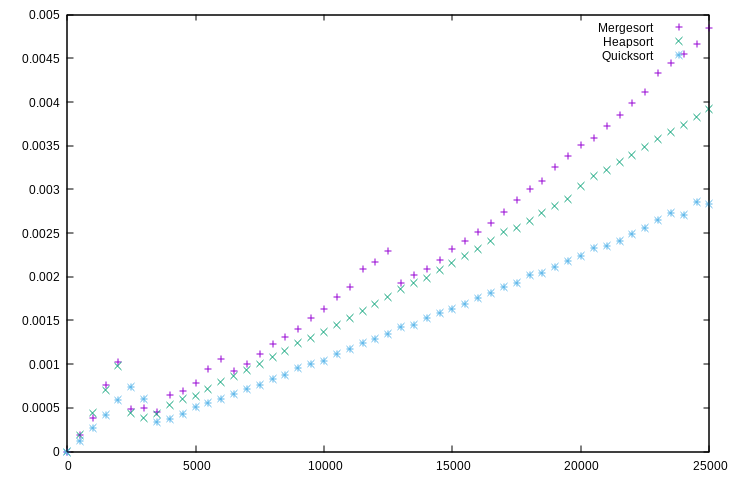
\includegraphics[totalheight=8cm]{img/ordenacion_rapida}
		\caption{Comparación gráfica del rendimiento de los algoritmos de ordenación rápida}
		\label{fig:ordenacion_rapida}
		\end{figure}
		\
	\subsubsection{Ordenación lentos}
		Estos algoritmos de ordenación, menos sofisticados, son de orden $O(n ^2)$ es decir, cuadráticos.
		\begin{longtable}{|c|c|c|c|}
			\hline
			Tamaño del vector & Tiempo con Burbuja & Tiempo con Selección & Tiempo con Inserción \\ \hline
			500	   &    0.00178596	&  0.00147628  	   &  0.00114028   \\ \hline
			1000  &	    0.0028655	&  0.0022588  	   &  0.00172961   \\ \hline
			1500  &	    0.00448784	&  0.00309903  	   &  0.00230721   \\ \hline
			2000  &	    0.00786624	&  0.00525987  	   &  0.00405115   \\ \hline
			2500  &	    0.0124692	&  0.00811555  	   &  0.00630397   \\ \hline
			3000  &	    0.0181514	&  0.0116717  	   &  0.00910679   \\ \hline
			3500  &	    0.0252785	&  0.0157854  	   &  0.0125022   \\ \hline
			4000  &	    0.0337448	&  0.0205625  	   &  0.0158871   \\ \hline
			4500  &	    0.0436306	&  0.0268227  	   &  0.0201791   \\ \hline
			5000  &	    0.0551609	&  0.0331552  	   &  0.026194   \\ \hline
			5500  &	    0.0681233	&  0.0401148  	   &  0.030802   \\ \hline
			6000  &	    0.0824843	&  0.0467118  	   &  0.035932   \\ \hline
			6500  &	    0.0984357	&  0.0540054   	   &  0.042335   \\ \hline
			7000  &	    0.11589	    &  0.0626111   	   &  0.0497211   \\ \hline
			7500  &	    0.135017	&  0.0717969   	   &  0.0573054   \\ \hline
			8000  &	    0.155683	&  0.0817153   	   &  0.0657382   \\ \hline
			8500  &	    0.176902	&  0.0921947   	   &  0.0768291   \\ \hline
			9000  &	    0.199919	&  0.103297	       &  0.0861508   \\ \hline
			9500  &	    0.225075	&  0.115035	       &  0.0981397   \\ \hline
			10000  &	0.251881	&  0.127486	       &  0.103923   \\ \hline
			10500  &	0.279234	&  0.140492	       &  0.122772   \\ \hline
			11000  &	0.309941	&  0.154166	       &  0.131101   \\ \hline
			11500  &	0.34121	    &  0.171219	       &  0.142071   \\ \hline
			12000  &	0.371406	&  0.183355	       &  0.158711   \\ \hline
			12500  &	0.405278	&  0.198969	       &  0.168258   \\ \hline
			13000  &	0.441736	&  0.215243	       &  0.178126   \\ \hline
			13500  &	0.478529	&  0.232051	       &  0.195711   \\ \hline
			14000  &	0.517851	&  0.249406	       &  0.215179   \\ \hline
			14500  &	0.557069	&  0.26754	       &  0.223471   \\ \hline
			15000  &	0.623507	&  0.286271	       &  0.245298   \\ \hline
			15500  &	0.64346	    &  0.305662	       &  0.257939   \\ \hline
			16000  &	0.693738	&  0.325702	       &  0.277471   \\ \hline
			16500  &	0.734539	&  0.346204	       &  0.297803   \\ \hline
			17000  &	0.778796	&  0.367458	       &  0.311583   \\ \hline
			17500  &	0.829418	&  0.39475	       &  0.322414   \\ \hline
			18000  &	0.880487	&  0.412826	       &  0.352076   \\ \hline
			18500  &	0.933294	&  0.435126	       &  0.360694   \\ \hline
			19000  &	0.986121	&  0.460939	       &  0.379935   \\ \hline
			19500  &	1.07066	    &  0.483263	       &  0.396013   \\ \hline
			20000  &	1.09964	    &  0.515923	       &  0.421674   \\ \hline
			20500  &	1.15639	    &  0.544332	       &  0.447574   \\ \hline
			21000  &	1.22045	    &  0.5604	       &  0.471736   \\ \hline
			21500  &	1.32645	    &  0.590167	       &  0.483069   \\ \hline
			22000  &	1.39171	    &  0.618805	       &  0.504104   \\ \hline
			22500  &	1.55601	    &  0.646724	       &  0.53811   \\ \hline
			23000  &	1.52041	    &  0.671924	       &  0.56646   \\ \hline
			23500  &	1.60414	    &  0.701547	       &  0.596336   \\ \hline
			24000  &	1.6872	    &  0.745452	       &  0.613182   \\ \hline
			24500  &	1.7148	    &  0.770377	       &  0.635088   \\ \hline
			25000  &	1.78348	    &  0.79409	       &  0.638414   \\ \hline
		\end{longtable}
	\begin{figure}[H]
		\centering
		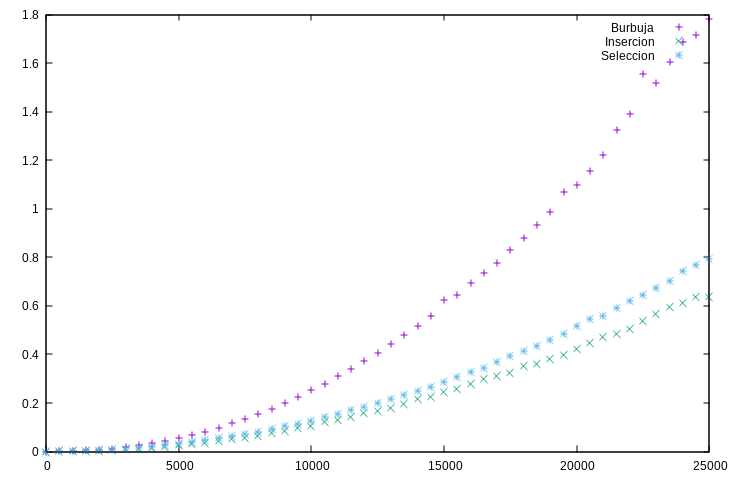
\includegraphics[totalheight=8cm]{img/ordenacion_lenta}
		\caption{Comparación gráfica del rendimiento de los algoritmos de ordenación lenta}
		\label{fig:ordenacion_lenta}
	\end{figure}
Por último, en las figuras \ref{fig:ordenacion} y \ref{fig:ordenacion_zoom}, se muestra el rendimiento de todos los algoritmos de ordenación, rápidos y lentos.
	\begin{figure}[H]
		\centering
		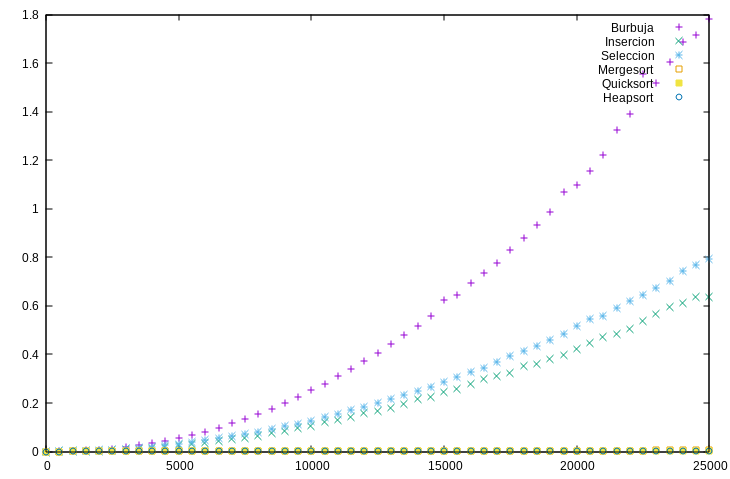
\includegraphics[totalheight=8cm]{img/ordenacion}
		\caption{Comparación gráfica del rendimiento de los algoritmos de ordenación}
		\label{fig:ordenacion}
	\end{figure}
	\begin{figure}[H]
		\centering
		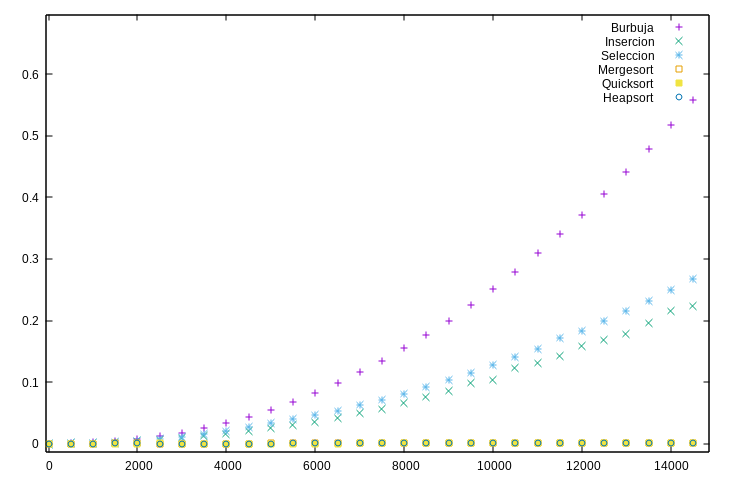
\includegraphics[totalheight=8cm]{img/ordenacion_zoom}
		\caption{\textit{Zoom} en el intervalo [0-15000] de la figura \ref{fig:ordenacion}}
		\label{fig:ordenacion_zoom}
	\end{figure}
\subsection{Floyd}
Dado un conjunto de nodos de un grafo dirigido, el algoritmo de Floyd calcula el costo del camino mínimo entre cada par. Pertenece al orden de eficiencia $O(n ^3)$, se muestra una gráfica en la figura \ref{fig:floyd}.
% TODO: Tabla con los tiempos de Floyd
\begin{figure}[H]
	\centering
	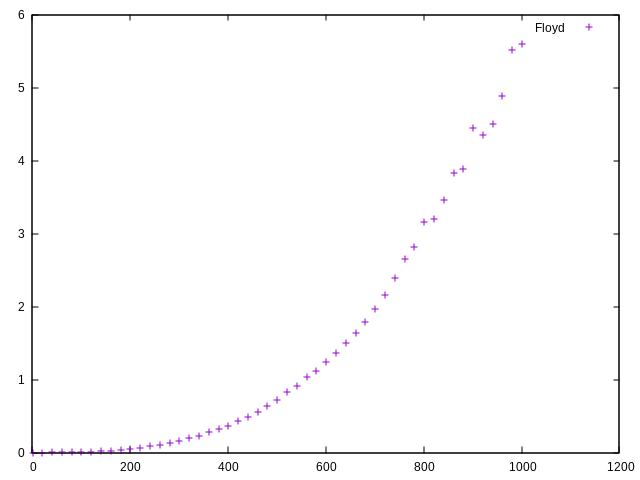
\includegraphics[totalheight=8cm]{img/floyd}
	\caption{Tiempos de ejecución en el algoritmo de Floyd}
	\label{fig:floyd}
\end{figure}
\subsection{Fibonacci}
Este algoritmo calcula los números de la sucesión de Fibonacci. 
\

Hace uso de la recursión y como hemos visto en clase, esto puede derivar muy facilmente en un algoritmo de orden exponencial, es este uno de esos casos.
\

$fib(n) \in O((\frac{1+\sqrt5}{2})^n)$

%TODO: Tabla con los tiempos de Fibonacci

\begin{figure}[H]
	\centering
	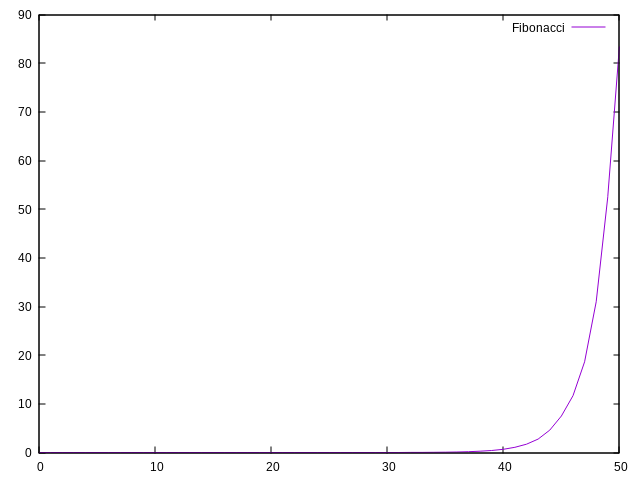
\includegraphics[totalheight=8cm]{img/fibonacci}
	\caption{Tiempos de ejecución en el algoritmo de Fibonacci}
	\label{fig:fibonacci}
\end{figure}

\subsection{Probando en distintas condiciones}
\subsubsection{Distintos ordenadores}
Hemos probado la misma implementación de un algoritmo en dos ordenadores distintos y así de paso demostrar el principio de invarianza.
\

En la figura \ref{fig:compSeleccion} se muestran los tiempos de ambos ordenadores en la misma gráfica y en la figura \ref{fig:compSeleccion_cociente}, la función cociente entre los tiempos de las dos ejecuciones.
\begin{figure}[H]
	\centering
	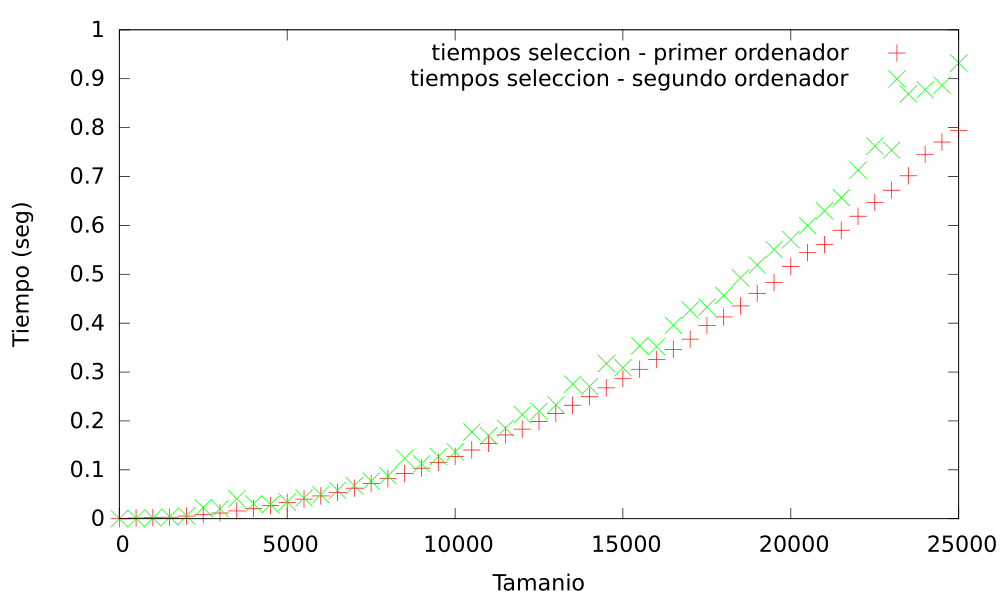
\includegraphics[totalheight=8cm]{img/compSeleccion}
	\caption{Equipos diferentes, tiempos distintos}
	\label{fig:compSeleccion}
\end{figure}
\begin{figure}[H]
	\centering
	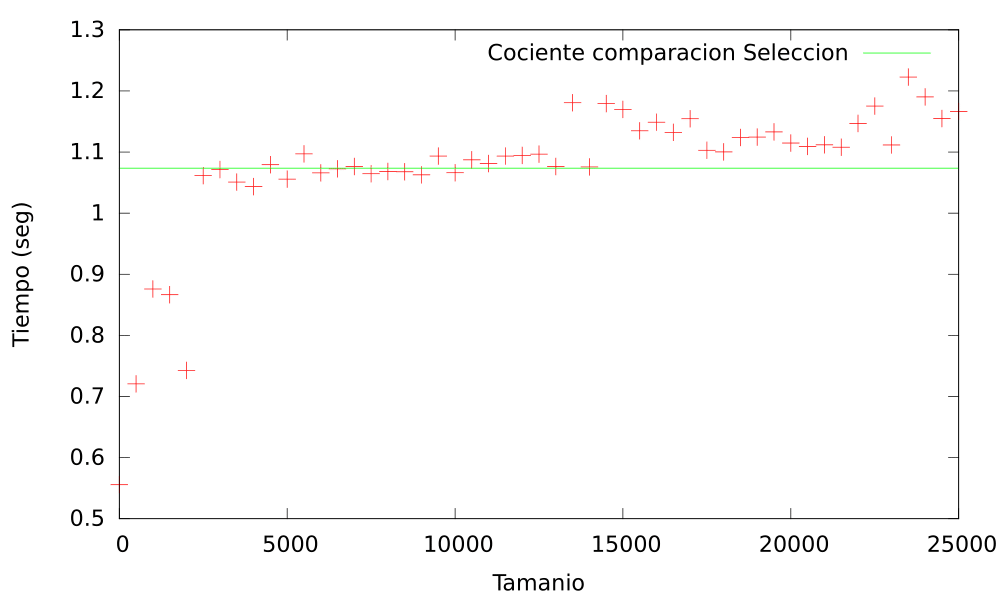
\includegraphics[totalheight=8cm]{img/compSeleccion_cociente}
	\caption{Demostrando el principio de invarianza}
	\label{fig:compSeleccion_cociente}
\end{figure}
\subsubsection{Distintas opciones de compilación}
En este caso hemos probado el algoritmo de Floyd en el mismo equipo, pero compilando con y sin optimización. (Hemos utilizado el \textit{switch} -O3 para la versión optimizada).

\begin{figure}[H]
	\centering
	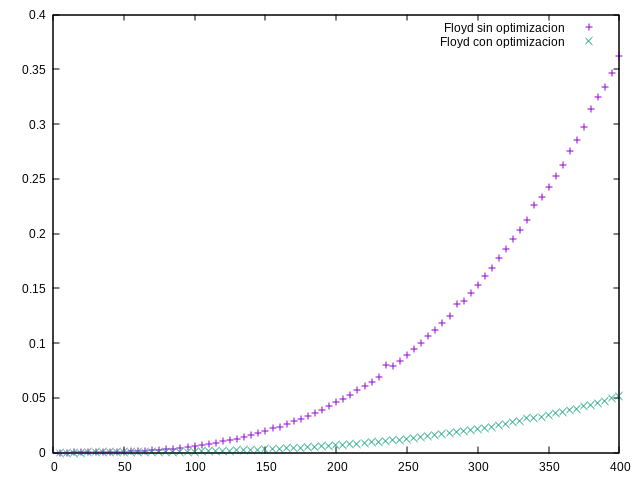
\includegraphics[totalheight=8cm]{img/optimizacion_floyd}
	\caption{Tiempos de ejecución compilando con y sin optimización}
	\label{fig:optimizacion_floyd}
\end{figure}

A pesar de todo, como se muestra en la figura \ref{fig:optimizacion_cociente}, sólo se diferencian en una constante $k \approx 0.141 $.
\begin{figure}[H]
	\centering
	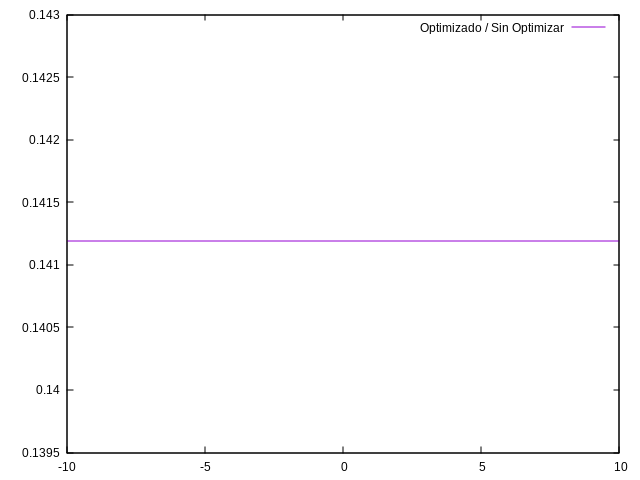
\includegraphics[totalheight=8cm]{img/optimizacion_cociente}
	\caption{El principio de invarianza, esta vez aplicado a las opciones del compilador.}
	\label{fig:optimizacion_cociente}
\end{figure}
%TODO: Estaría bien una tercera subsubsection con algo que se os ocurra

\section{Eficiencia híbrida}
%TODO: Esto
\end{document}
